%%%%%%%%%%%%%%%%%%%%%%%%%%%%%%%%%%%%%%%%%
% Paper 1 --- funder deliverable draft
% Framing: methods paper + demonstration (not a regional case-study
% product). Primary contribution = transferable backtest design,
% contrast, and scoring; secondary = what four Celtic/Irish Sea
% gadoids show under that design.
% Locked identity: one treatment (closed-loop ICES Category 1 advice
% rule vs historical realised F). Constant published ICES F_MSY open
% loop is a no-feedback benchmark only (column in tab:results-current;
% not a co-equal policy). Benchmark series is labelled "open-loop F_MSY"
% (never F_target, which is the HCR control point). Open-loop uses
% published ICES F_MSY = Ftar.
% Scope of this PDF: perfect-information residual-replay backtest
% (true OM SSB, implErr=0, reference OM bh3). Demonstration stocks:
% four gadoids (Celtic/Irish Sea cod and whiting). Peer-review upgrades
% (multiple OMs; OEM for CPUE; SAM inside the MP) are listed only in
% section Next steps --- not claimed in Methods/Results.
% Companion: abstract.tex, code-to-run.md, supplementary.tex.
% Existing six-stock draft left intact in paper.tex (do not mix).
% Results tables use provisional numbers from the deterministic
% reference-OM run (paper.tex / 06.0_report.Rmd); figures use existing
% SI and report knits (freeze on re-knit if needed).
%%%%%%%%%%%%%%%%%%%%%%%%%%%%%%%%%%%%%%%%%
%!TEX program = xelatex
\documentclass[11pt,a4paper]{article}

\usepackage[margin=2.5cm]{geometry}
\usepackage{amsmath,amssymb}
\usepackage{booktabs}
\usepackage{graphicx}
\usepackage{setspace}
\usepackage{natbib}
\usepackage{tikz}
\usetikzlibrary{arrows.meta,positioning,calc}
\usepackage{hyperref}
\onehalfspacing
\setlength{\parindent}{0pt}
\setlength{\parskip}{0.5em}

\newcommand{\Fmsy}{F_{\mathrm{MSY}}}
\newcommand{\Blim}{B_{\lim}}
\newcommand{\Btrig}{\mathrm{MSY}_{B_{\mathrm{trigger}}}}
\newcommand{\Bmsy}{B_{\mathrm{MSY}}}
\newcommand{\Ftar}{F_{\mathrm{target}}}

\title{Separating advice-rule performance from implementation and
productivity: a historical closed-loop backtest\thanks{Alternative
(regional) title: A backtest of the ICES Category~1 advice rule for
Celtic and Irish Sea gadoids.}}
\author{}
\date{}

\begin{document}
\maketitle

%------------------------------------------------------------------------------
% Paper 1 abstract (ICES JMS / Fish and Fisheries style).
% Framing: methods paper + demonstration (not a regional case-study product).
% Locked identity: one treatment (closed-loop ICES Category 1 advice
% rule vs historical realised F) + one no-feedback benchmark (constant
% published ICES F_MSY = Ftar). Demonstration: four gadoids
% (Celtic/Irish Sea cod and whiting); OM = reference Beverton--Holt (bh3).
% Scope: perfect-information residual-replay backtest (funder deliverable).
% Do not \input this into paper.tex until that draft is retired;
% paper.tex still carries the six-stock (incl. mackerel) working-paper abstract.
%
% Title (locked; set in skeleton.tex):
%   Separating advice-rule performance from implementation and
%   productivity: a historical closed-loop backtest
% Alternative (regional; carried as \thanks in skeleton.tex):
%   A backtest of the ICES Category 1 advice rule for Celtic and
%   Irish Sea gadoids
%
\begin{abstract}
Realised stock trajectories confound fishing, environmental variability,
and the performance of advice frameworks. Retrospective analysis and
management strategy evaluation (MSE) leave a gap: neither isolates an
advice rule from implementation under the productivity that actually
occurred. We present a historical closed-loop \emph{backtest} that holds
observed productivity fixed in an age-structured operating model,
contrasts perfect closed-loop implementation of a harvest control rule
(HCR), as coded, with historical realised fishing mortality, and scores
outcomes against both operational control points and operating-model (OM)
reference points. A constant open-loop path at the published ICES
$F_{\mathrm{MSY}}$ (equal to $\Ftar$ in the advice rule) is retained
only as a no-feedback benchmark. We demonstrate the design with four ICES
Category~1 gadoids in the Celtic and Irish Seas---Celtic Sea cod, Irish
Sea whiting, Irish Sea cod, and Celtic Sea whiting---under perfect
information (true OM SSB; residual replay; zero implementation error)
with the ICES $\pm20\%$ TAC stability clause above $\Btrig$.
Across the four stocks, three outcome patterns emerge:
following the rule would have rebuilt stocks that were subject to
overfishing (realised $F$ above the target fishing mortality $\Ftar$);
the opposite can occur where realised $F$ already sat below $\Ftar$; and
the two yardsticks---ICES control points such as $\Btrig$ and OM MSY
reference points---can disagree, so that a stock scored as rebuilt
against OM MSY biomass may never clear $\Btrig$ under the rule, with the
size of the gap set by the OM stock--recruitment relationship.
\end{abstract}

\noindent\textit{Keywords:} advice; harvest control rule; backtest; maximum sustainable yield; management strategy evaluation; productivity; gadoids.

%------------------------------------------------------------------------------

%==============================================================================
\section{Introduction}
\label{sec:intro}
%==============================================================================

A main objective when providing advice for many commercially targeted stocks
is to achieve the maximum sustainable yield (MSY). An objective that is increasingly implemented through the use of harvest control rule (HCRs) with operational control points corresponding to a target fishing mortality ($\Ftar$), a biomass threshold ($\Btrig$) below which $F$ is reduced, and a biomass limit ($\Blim$) that the rule is intended to avoid with high probability. These are operational control points rather than biological targets, for example in the ICES advice rule, $\Btrig$ is not $\Bmsy$, and $\Ftar$ need not coincide with $\Fmsy$. However, managers and the public often treat being above $\Btrig$ as achieving the ``MSY'' objective \citep{winker2026rebuilding}.

Even when advice is based on a HCR designed to achieve $MSY$ while ensuring that they is a low probability of a stock being depleted to a level where productivity is impaired, stocks may be assessed as being overfished. This is often attributed to environmental change. However, an historical assessment alone
cannot separate between three potential explanations: that the HCR was faithfully
implemented but failed; that the HCR was not followed; or that productivity was
unfavourable. However, attribution is problematic.

A standard diagnostic in stock assessment is retrospective analysis, this evaluates the consistency of assessment estimates as data accumulate \citep{mohn1999}; it does not however evaluate HCR performance. HCRs are normally developed through Management Strategy Evaluation \citep[MSE][]{punt2016msebestpractice} which evaluates candidate strategies as a closed loop simulation (i.e. with feedback) for hypothetical futures. Neither, however, isolates the advice rule from implementation under the productivity that actually occurred. Therefore  we conduct a closed-loop historical simulation, i.e. a backtest. as a counterfactual. This is based on an age-structured Operating Model (OM), conditioned on the most recent assessment that asks what would have happened if advice had been followed, holding observed productivity fixed (by using year-specific biology and replaying stock--recruitment residuals) and contrasting the advice rule with historical estimates of fishing mortality, spawning stock biomass. and catch.

The study asks two questions. First, would following the advice rule
have resulted in a different stock status, given the productivity that actually occurred? Second, does the answer depend on the benchmark used, i.e. the ICES control points ($\Btrig$, $\Ftar$) or the MSY reference points from the OM ($\Bmsy$, $\Fmsy$)? To answer these questions, we replay the historical period with productivity held fixed. The rule is applied year--by--year,
so each year's advice responds to the simulated stock (a closed loop),
and the result is compared with outcomes based on the historical fishing mortality. As a benchmark the stock was also projected at a constant level of $F$ equal to the published ICES $F_{\mathrm{MSY}}$ (the same value as $\Ftar$ in the advice rule) with no feedback (an open loop).

The approach is generic and can be applied to any stock where advice is based on a HCR by conditioning an OM on a stock-assessment. We demonstrate the design with four ICES Category~1 gadoids in the Celtic and Irish Seas; Celtic Sea cod, Irish Sea whiting, Irish Sea cod, and Celtic Sea whiting (Table~\ref{tab:casestudy-status}; Figure~\ref{fig:advice-catch}). Celtic Sea cod and Irish Sea whiting are currently subject to overfishing as $F$ is above $\Ftar$, and is overfished as SSB is below $\Blim$. For Irish Sea cod, $F$ has been below $\Ftar$ since 2000, yet SSB has declined and is currently below $\Blim$. Celtic Sea whiting was fished above $\Ftar$ over the backtest window but is below it in the latest assessment year, and currently remains below $\Blim$. For these stocks we ask whether applying the Category~1 rule exactly would have changed their status in the terminal year, and whether being above $\Btrig$ means that MSY objectives are met in the OM.

%==============================================================================
\section{Materials and methods}
\label{sec:methods}
%==============================================================================

The backtest conditions an age-structured OM on the latest assessment, then reuses historical mass, maturity and selectivity-at-age and projects across the backtest years for the assumed stock--recruitment relationship, replaying the recruitment deviations. This maintains the observed productivity, as the HCR is applied each advice year. The ICES reference points from the Stock Assessment Graphs database
(SAG) are used by the HCR. The OM value of $\Bmsy$ is a performance metric. This is not a conventional MSE of unobserved futures. Stock-specific conditioning, start years, and status summaries for the demonstration are given in Section~\ref{sec:demo-stocks}.

\paragraph{Notation.} $\Ftar$ is the HCR target (ICES Category~1
control point); $\Fmsy$ and $\Bmsy$ are OM MSY reference points and are
not equated with the advice-rule targets. In the open-loop benchmark,
published ICES $F_{\mathrm{MSY}}$ is used as the constant $F$ and equals
$\Ftar$ in the advice rule.

\subsection{Advice framework and diagnostic hierarchy}
\label{sec:diag-hierarchy}

The diagnostic procedures used in stock assessment include retrospective analysis of the consistency of estimates, and hindcast cross-validation of prediction skill of observations \citep{Carvalho2021cookbook}. While MSE tests candidate management strategies, that includes monitoring, assessment, and  management actions, in closed loop against a
simulated OM that represents the stock and fishery \citep{punt2016msebestpractice}. Here we combine the approaches  by backtesting a strategy against management
objectives under historical conditions. We ask whether the advice rule would have met its objectives given the productivity that occurred not whether the rule is robust under climate regimes that have not been observed.

The backtest is a perfect-information short-cut: an age-structured OM is
conditioned on the latest assessment, and observed productivity
(year-specific biology plus stock--recruitment residuals) is replayed
inside that OM. Each advice year the HCR is applied to true OM SSB, and
the resulting catch is taken without implementation error. The simulated
SSB, $F$, and catch are then compared with the realised assessment
trajectories. There is no assessment re-fit inside the loop.

\begin{figure}[htbp]
\centering
% Design schematic for the historical closed-loop backtest
% (OM -- three arms -- score). Self-contained TikZ;
% requires \usepackage{tikz} and \usetikzlibrary{arrows.meta,positioning,calc}.
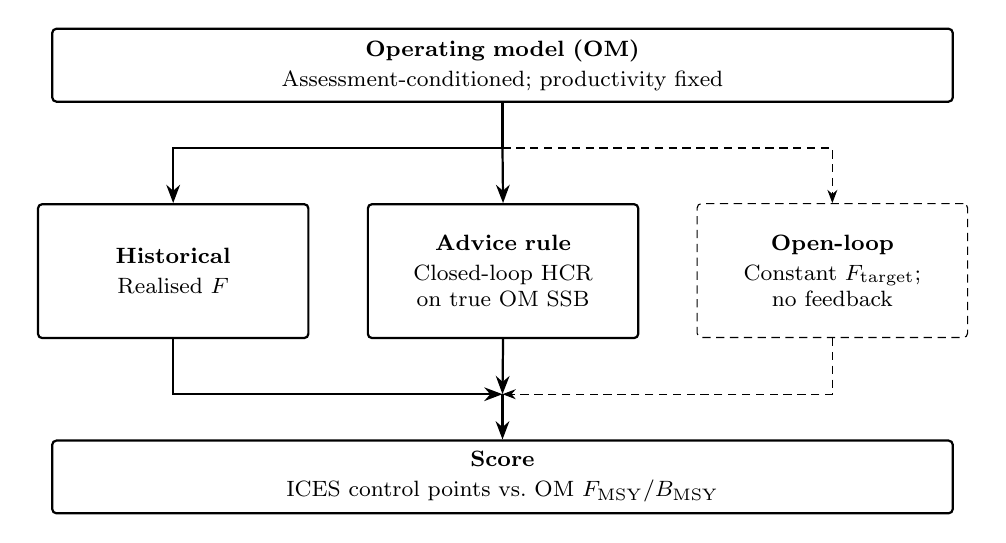
\begin{tikzpicture}[
  font=\footnotesize,
  >=Stealth,
  box/.style={
    draw, thick, rounded corners=1.5pt,
    align=center, inner sep=4pt
  },
  wide/.style={box, text width=0.92\linewidth},
  arm/.style={box, text width=0.26\linewidth, minimum height=1.7cm},
  armdash/.style={arm, densely dashed, thin},
  arr/.style={->, thick}
]
  % Operating model
  \node[wide] (om) {%
    \textbf{Operating model (OM)}\\[0.15em]
    Assessment-conditioned; productivity fixed};

  % Three contrast arms in a matrix (guaranteed equal gap, no overlap)
  \matrix[
    below=1.15cm of om,
    column sep=0.06\linewidth,
    ampersand replacement=\&
  ] (arms) {
    \node[arm] (hist) {%
      \textbf{Historical}\\[0.15em]
      Realised $F$}; \&
    \node[arm] (advice) {%
      \textbf{Advice rule}\\[0.15em]
      Closed-loop HCR\\
      on true OM SSB}; \&
    \node[armdash] (open) {%
      \textbf{Open-loop}\\[0.15em]
      Constant $\Ftar$;\\
      no feedback}; \\
  };

  \coordinate (fork) at ($(om.south)!0.5!(arms.north)$);
  \draw[thick] (om.south) -- (fork);
  \draw[arr] (fork) -| (hist.north);
  \draw[arr] (fork) -- (advice.north);
  \draw[arr, densely dashed, thin] (fork) -| (open.north);

  % Dual scoring
  \node[wide, below=1.15cm of arms] (score) {%
    \textbf{Score}\\[0.15em]
    ICES control points vs.\ OM $\Fmsy$/$\Bmsy$};

  \coordinate (join) at ($(arms.south)!0.5!(score.north)$);
  \draw[arr] (hist.south) |- (join);
  \draw[arr] (advice.south) -- (join);
  \draw[arr, densely dashed, thin] (open.south) |- (join);
  \draw[arr] (join) -- (score.north);

\end{tikzpicture}

\caption{Design of the historical closed-loop backtest. An
assessment-conditioned OM holds productivity fixed. The policy contrast is
\emph{Historical} realised $F$ versus a closed-loop HCR on true OM SSB
(perfect-information short-cut). A subordinate open-loop series holds
published ICES $F_{\mathrm{MSY}}$ ($=\Ftar$ in the advice rule) constant
with no feedback. Outcomes are scored against ICES control points and OM
reference points ($\Fmsy$, $\Bmsy$).}
\label{fig:design}
\end{figure}

\subsection{Operating model}

The OMs are conditioned on the latest ICES assessment for each stock. In the historical window the forward projection retains the assessed time series of weights, natural mortality, maturity, and selectivity. Results reported here use a Beverton--Holt stock--recruitment relationship
\citep{beverton1957dynamics} (hereafter the reference OM) fitted with a
tight prior (CV $=0.001$) on virgin recruitment $R_0$, whose prior value
is set, as coded, from the ratio $\Btrig/\Blim$ of the published ICES
reference points.
% FLAG (dimensional check): 02.0_condition_om.Rmd (bh3) passes
% prior_r0 = MSYBtrigger/Blim (dimensionless, ~1.39) with cv_r0 = 0.001
% to icesdata::eql(model="bevholtSV"). R0 is in recruits, so confirm
% whether eql rescales prior_r0 (e.g. relative to mean recruitment or on
% a log/relative scale) before describing this as a prior "on R0".
% Not resolved from the code; wording above only states what is coded.
HCR control points remain the published ICES values ($\Ftar$, $\Blim$,
and $\Btrig$). The hockey-stick is not re-targeted to OM reference
points, nor is the ICES hockey-stick treated as biological truth; it is
the advice-rule shape and the source of the reference-OM $R_0$ prior
value only.
% Code: OM branch bh3 in eqls; control points on eqls[["bh1"]] (eqs,
% via addBenchmark). Conditioning in Rmd/02.0_condition_om.Rmd.

Multiplicative deviations from the reference-OM stock--recruitment
relationship are replayed with a single iteration: a deterministic
residual history. That fixed productivity is what makes the Historical
versus Advice-rule contrast interpretable.

\subsection{Advice rule}
\label{sec:hcr}

The experiment has one harvest-policy contrast: the closed-loop ICES
Category~1 advice rule versus historical realised $F$. A third
trajectory---open-loop projection at the published ICES
$F_{\mathrm{MSY}}$ (equal to $\Ftar$ in the advice rule) without
biomass feedback, labelled open-loop $\Fmsy$ in figures and tables---is
computed only as a no-feedback reference; that constant is the
advice-rule target, not OM $\Fmsy$. All three share the same OM biology
and residual replay; only the $F$ process differs.

\paragraph{Closed loop}
For each advice year $t$ from 2015 to the stock's terminal year, the
management procedure (i)~perceives status from true OM SSB in the last
simulated year, (ii)~applies the ICES HCR to set $F$ and thence catch for
$t{+}1$, (iii)~implements that catch on the OM with zero implementation
error, and (iv)~compares SSB, $F$, and catch with the realised
assessment. The run uses residual deviations from the reference-OM
relationship, annual advice, and no year-to-year TAC bounds.
% Code: err=NULL, implErr=0, interval=1, bndTac=c(0,Inf).

\paragraph{HCR}
Operational control points follow the generic harvest-control-rule framing
of \citet{winker2026rebuilding}: a target fishing mortality ($\Ftar$), a
biomass trigger below which $F$ is reduced, and a biomass limit ($\Blim$)
that the advice framework is intended to avoid with high probability. In
ICES Category~1 advice the trigger is $\Btrig$ (which maps to
$B_{\mathrm{trigger}}$ in that generic HCR). When biomass is above the
trigger, exploitation proceeds at $\Ftar$; as biomass declines below it,
harvest rates become progressively more restrictive. Control points are
$\Ftar$ (the published ICES $F_{\mathrm{MSY}}$ used as the advice-rule
target), trigger $\Btrig$, $B_{\min}=0$, and
$F_{\min}=0.05\,\Ftar$. The implemented hockey-stick is
\begin{equation}
  F_{\mathrm{advice}}(B)
  \;=\;
  \begin{cases}
  \Ftar
    & \text{if } B \ge \Btrig,\\[0.35em]
  F_{\min}
    + (\Ftar - F_{\min})\,
      \dfrac{B - B_{\min}}{\Btrig - B_{\min}}
    & \text{if } B_{\min} < B < \Btrig,\\[0.75em]
  F_{\min}
    & \text{if } B \le B_{\min},
  \end{cases}
  \label{eq:hcr}
\end{equation}
so the slope runs from $(B_{\min},F_{\min})$ to $(\Btrig,\Ftar)$, not from
$\Blim$ to $\Btrig$: a closure at $\Blim$ is not imposed ($F_{\min}>0$).
Catch advice is a one-year forward projection at $F_{\mathrm{advice}}$.
Published $\Blim$ remains an evaluation threshold for status and scoring,
not the breakpoint of eq.~\eqref{eq:hcr}. The treatment is therefore the
ICES Category~1 MSY rule \emph{as coded} ($F_{\min}=0.05\,\Ftar$, no
closure below $\Blim$). It can differ from advice as issued, which may,
for example, recommend zero catch when SSB is below $\Blim$.
% Code: hcrParams on eqs (SAG on bh1); F_min is the FLBRP-method default.

\paragraph{Benchmark}
\emph{Historical} is the latest WGCSE assessment: realised $F$, catch,
and SSB as assessed, against which the counterfactual is scored.
\emph{Advice rule} is the closed-loop treatment above---the only
``perfect implementation'' claim in this deliverable. The
\emph{open-loop $\Fmsy$} series is a forward projection at constant
published ICES $F_{\mathrm{MSY}}$ (equal to $\Ftar$) from about 1990 to
the terminal year: no SSB feedback and no reduction of $F$ when biomass
is below $\Btrig$. It answers only ``what if fishing had been held at
the published ICES $F_{\mathrm{MSY}}$ with no hockey-stick''. Start years
differ by design: the HCR backtest covers the modern Category~1 MSY rule
from 2015, whereas the open-loop series is a long constant-$F$
reference, not a contemporaneous advice reconstruction. The open-loop
series is therefore a no-feedback reference, and comparing it with the
Advice rule is not a clean isolation of HCR shape: terminal differences
mix rule shape with 25 years of different fishing history before 2015.
The results table (Table~\ref{tab:results-current}) reports Historical,
open-loop $\Fmsy$ (benchmark), and Advice rule; the headline $\Delta$ is
Advice rule minus Historical $\mathrm{SSB}/\Btrig$ only. The published
ICES $F_{\mathrm{MSY}}$ is itself derived from open-loop simulation
(EqSim), so the constant-$F$ projection is its no-feedback analogue
rather than a closed-loop test of the advice rule
\citep{winker2025precautionary}.
% Code: open-loop start = openloop_start (1990, or two years after the
% first assessment year if later).

\subsection{Projection}
Over the historical years, year-specific $M$, mass, and maturity,
together with stock--recruitment residuals, are held common across the
Advice-rule run and the open-loop $\Fmsy$ benchmark. Same productivity
and different $F$ processes are what make the contrast interpretable. We
refer to the period from 2015 to each stock's terminal year as the
\emph{backtest window}; metrics summarising it are labelled
\emph{Current}.

After the terminal year, a 20-year projection (labelled \emph{Future}) is
started from the Historical and Advice-rule terminal states only. No
Future is projected from the open-loop benchmark. The Future uses mean
biology from the equilibrium object, recruitment deviations equal to one
(mean productivity, not a continuation of the residual history), and the
same ICES HCR. It is longer than an ICES one- to two-year advice forecast
and is not a stochastic climate projection.
% Code: Rmd/04.3_rebuild.Rmd.

\subsection{Evaluation}

Two roles for reference points are kept distinct. ICES $\Ftar$, $\Blim$,
and $\Btrig$ are operational control points of the advice rule, held
fixed from SAG. OM $\Bmsy$ and $\Fmsy$ are performance metrics from the
reference OM. Headline Current metrics (Table~\ref{tab:results-current})
are terminal $\mathrm{SSB}/\Btrig$, mean $F$, and mean $F/\Ftar$ over the
backtest window under Historical, the open-loop $\Fmsy$ benchmark, and
the Advice rule, with $\Delta$ equal to Advice-rule minus Historical
$\mathrm{SSB}/\Btrig$. Future metrics (Table~\ref{tab:results-future})
are years from each of the Historical and Advice-rule terminal states to
ICES $\Btrig$ and to OM $\Bmsy$: zero if already above the threshold, and
missing if not reached within twenty years. Probabilities such as
$P(\mathrm{SSB}<\Blim)$, mean yield, and inter-annual catch variability
are standard MSE-style summaries but are not the headline for this
deterministic residual replay.

\paragraph{Software}
Analyses use the FLR packages FLCore, FLBRP, and FLasher
\citep{Kell2007FLR}; the FLBacktest package for the advice rule, the
open-loop and closed-loop projections, and the OM gate
\citep{FLBacktestMethods}; and icesdata for conditioning and SAG
reference points.

\subsection{Demonstration stocks}
\label{sec:demo-stocks}

The demonstration uses four Celtic and Irish Sea gadoids under the ICES
MSY advice basis: Celtic Sea cod (\texttt{cod.27.7e-k}), Irish Sea
whiting (\texttt{whg.27.7a}), Irish Sea cod (\texttt{cod.27.7a}), and
Celtic Sea whiting (\texttt{whg.27.7b-ce-k}). Terminal years of the
cleaned WGCSE assessments used to condition the OMs are 2023 (Irish Sea
cod and whiting), 2024 (Celtic Sea whiting), and 2025 (Celtic Sea cod).
The closed-loop treatment starts in 2015. The open-loop $\Fmsy$ benchmark
starts in 1990, or two years after the first assessment year if later.
The exercise is a counterfactual backtest, not a statutory re-assessment
of advice.
% Inventory: data/reference/stocks.csv.

Initial screening compares ICES advised catch from the Advice and
Scenarios Database (ASD) with reported catch from the latest SAG
assessment year (Figure~\ref{fig:advice-catch}). Years in which reported
catch exceeds advice mark an implementation gap, so depleted terminal
status alone cannot distinguish advice not followed from HCR failure
under the productivity that occurred.

\begin{figure}[htbp]
\centering
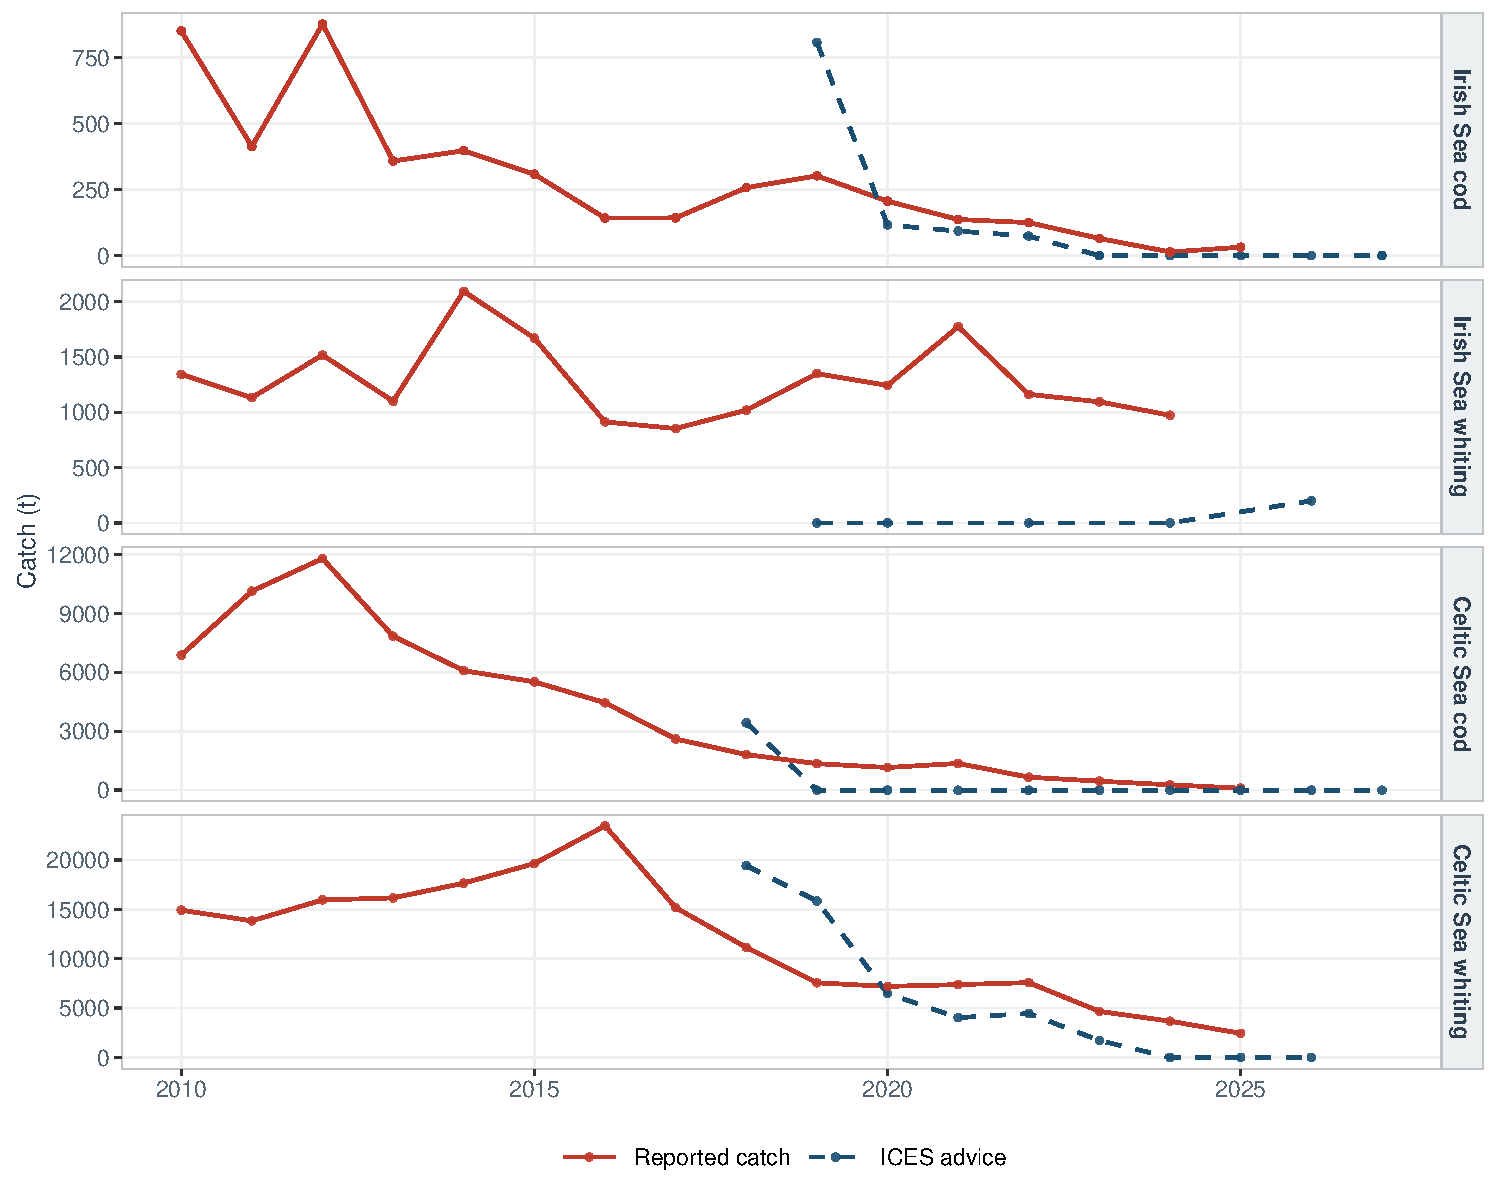
\includegraphics[width=\textwidth]{figs/advice_catch_casestudy.pdf}
\caption{ICES advised catch (ASD) and reported catch (SAG) for the four
demonstration stocks, 2010 onward. Facets use independent $y$-axes
(tonnes).}
\label{fig:advice-catch}
\end{figure}
% Source: Rmd/01_screening.Rmd (S3.2 ICES advice vs reported catch).

SAG screening places all four stocks below $\Blim$ in the latest
assessment year (Table~\ref{tab:casestudy-status}): Celtic Sea cod and
Irish Sea whiting with $F/\Ftar>1$; Irish Sea cod and Celtic Sea whiting
with $F/\Ftar<1$. These are terminal-year values from the latest SAG
assessment; for Celtic Sea whiting the mean over the backtest window was
above $\Ftar$ (Section~\ref{sec:res-scoring}). The terminal-year contrast
frames the Historical versus Advice-rule comparisons below and
anticipates the outcome patterns in Section~\ref{sec:results}.

\begin{table}[htbp]
\centering
\caption{Latest SAG terminal-year status for the four demonstration
stocks. Ratios use published ICES $\Blim$, $\Btrig$, and $\Ftar$.
Values are from the latest SAG assessment (column ``Ass.''), which can be
a later vintage than the WGCSE assessment used to condition the OM (e.g.\
Irish Sea cod: SAG terminal year 2026; conditioning assessment ends
2023). Absolute SSB, $F$, and reference-point values are in the
supplementary status table.}
\label{tab:casestudy-status}
\begin{tabular}{@{}lrrrrr@{}}
\toprule
Stock & Ass. & Year &
  SSB/$\Btrig$ & SSB/$\Blim$ & $F/\Ftar$ \\
\midrule
Celtic Sea cod     & 2026 & 2025 & 0.02 & 0.02 & 4.95 \\
Irish Sea whiting  & 2025 & 2024 & 0.53 & 0.73 & 4.14 \\
Irish Sea cod      & 2026 & 2026 & 0.28 & 0.38 & 0.05 \\
Celtic Sea whiting & 2026 & 2025 & 0.26 & 0.36 & 0.65 \\
\bottomrule
\end{tabular}
\end{table}
% Source: Rmd/01_screening.Rmd (S3.5 Latest stock status).

%==============================================================================
\section{Results}
\label{sec:results}
%==============================================================================

Results are from a single deterministic run of the reference OM under
perfect information. Numbers in the tables and prose match that run;
figures are existing knits and will be frozen from a re-knit if the
report notebook is refreshed. Results are organised by outcome pattern.

\subsection{Outcome pattern~1: overfishing relative to \texorpdfstring{$\Ftar$}{Ftarget}}
\label{sec:res-overfished}

Celtic Sea cod and Irish Sea whiting exemplify stocks where realised
$\bar F$ sat well above $\Ftar$ (Celtic Sea cod $F/\Ftar \approx 4.4$;
Irish Sea whiting $\approx 5.3$).
\begin{itemize}
  \item Advice rule vs history: terminal $SSB/\Btrig$ several times the
        trigger (cod $\approx 4.2$; whiting $\approx 4.9$);
        $\Delta \approx +4.2$ and $+4.4$.
  \item Benchmark check: the open-loop $\Fmsy$ trajectory moves in the
        same direction. Because it starts about 25 years earlier than
        the HCR, this is consistent with recovery being driven by fishing
        nearer $\Ftar$ rather than by the hockey-stick slope, but does
        not isolate the two.
  \item Following the ICES Category~1 rule as coded would have changed
        Current status for this outcome pattern
        (Figures~\ref{fig:hero} and~\ref{fig:hero-whg};
        Table~\ref{tab:results-current}).
  \item Future: Irish Sea whiting is already above both thresholds at the
        Advice-rule start (Figure~\ref{fig:hero-whg}); Celtic Sea cod is
        already above $\Btrig$ at the Advice-rule start but OM $\Bmsy$
        is not reached in 20 years from either start
        (Figure~\ref{fig:hero}; Table~\ref{tab:results-future};
        Section~\ref{sec:res-scoring}).
\end{itemize}

\subsection{Outcome pattern~2: opposite sign under light historical \texorpdfstring{$F$}{F}}
\label{sec:res-opposite}

Irish Sea cod exemplifies the opposite sign: Historical
$F/\Ftar \approx 0.07$, and the Advice rule \emph{lowers} terminal
$SSB/\Btrig$ ($\Delta \approx -0.21$).
\begin{itemize}
  \item Benchmark check: the open-loop $\Fmsy$ path shows the same
        sign, which is consistent with the effect coming from the level
        of $\Ftar$ rather than from the hockey-stick; the single-stock
        $F$ implied by $\Ftar$ is higher than realised $F$.
  \item This is not ``implementation failure'' in the same sense as
        Outcome pattern~1. Catch sat below what the single-stock
        Category~1 rule as coded would have allowed. Part of that gap
        may reflect advice as issued, which can be more restrictive than
        the coded rule below $\Blim$, rather than implementation. Other
        candidate mechanisms (mixed-fishery choke, recovery TACs, or a
        mismatch between $\Ftar$ and OM $\Fmsy$) are not identified here.
  \item Future: reaches OM $\Bmsy$ before ICES $\Btrig$ (6 vs 8 years
        from history) because OM $\Bmsy$ sits below $\Btrig$ in the
        reference OM (Figure~\ref{fig:pattern2}, right;
        Tables~\ref{tab:results-current} and~\ref{tab:results-future}).
\end{itemize}

\subsection{Outcome pattern~3: ICES control points and OM MSY reference points can disagree, in either direction}
\label{sec:res-scoring}

$\Btrig$ and OM $\Bmsy$ are different yardsticks, and in this
demonstration they disagree in both directions.
\begin{itemize}
  \item OM $\Bmsy$ above $\Btrig$ (clearing the trigger without reaching
        MSY biomass): Celtic Sea cod is already above $\Btrig$ at the
        Advice-rule start, yet OM $\Bmsy$ is not reached in 20 years
        from either start (Figure~\ref{fig:hero}, right;
        Table~\ref{tab:results-future}).
  \item OM $\Bmsy$ below $\Btrig$ (reaching MSY biomass while below
        trigger): for Celtic Sea whiting, mean $F/\Ftar$ over the
        backtest window was above target (Historical $1.42$), and the
        HCR cuts it to $0.63$, but terminal $SSB/\Btrig$ rises only from
        $0.22$ to $0.49$. In the Future it never reaches ICES $\Btrig$
        in 20 years from either start, yet reaches OM $\Bmsy$ in 16--18
        years (Figure~\ref{fig:pattern3};
        Table~\ref{tab:results-future}). Irish Sea cod shows the same
        direction (Figure~\ref{fig:pattern2}; Section~\ref{sec:res-opposite}).
  \item Benchmark check for Celtic Sea whiting: the open-loop $\Fmsy$
        path also stays below trigger (terminal $SSB/\Btrig \approx
        0.40$). Under this stock--recruitment relationship and these
        residuals, neither the rule as coded nor constant $\Ftar$
        clears $\Btrig$ by the terminal year; given the different start
        years, this is a diagnostic of the realised productivity against
        the ICES control points, not two policies both failing.
  \item A 20-year mean-recruitment HCR projection can therefore look
        like a successful rebuild against OM $\Bmsy$ while remaining
        ``below trigger'' on the ICES scale, and vice versa.
\end{itemize}

\begin{table}[htbp]
\centering
\caption{Current metrics for the four demonstration stocks: terminal
$SSB/\Btrig$, mean $\bar F$, and mean $\bar F/\Ftar$ over the backtest
window for Historical, open-loop $\Fmsy$ (no-feedback benchmark;
published ICES $F_{\mathrm{MSY}}=\Ftar$), and Advice rule (treatment),
plus $\Delta$ (Advice rule $-$ Historical $SSB/\Btrig$). Deterministic
reference-OM run.}
\label{tab:results-current}
\resizebox{\textwidth}{!}{%
\begin{tabular}{@{}l rrr rrr rrr r@{}}
\toprule
 & \multicolumn{3}{c}{Historical}
 & \multicolumn{3}{c}{Open-loop $\Fmsy$}
 & \multicolumn{3}{c}{Advice rule}
 & AR $-$ Hist \\
\cmidrule(lr){2-4}\cmidrule(lr){5-7}\cmidrule(lr){8-10}\cmidrule(lr){11-11}
Stock & $SSB/\Btrig$ & $F$ & $F/\Ftar$
      & $SSB/\Btrig$ & $F$ & $F/\Ftar$
      & $SSB/\Btrig$ & $F$ & $F/\Ftar$
      & $\Delta$ \\
\midrule
Celtic Sea cod     & 0.02 & 1.29 & 4.44 & 4.22 & 0.29 & 1 & 4.23 & 0.29 & 1.00 & 4.21 \\
Irish Sea whiting  & 0.51 & 1.10 & 5.25 & 4.94 & 0.21 & 1 & 4.95 & 0.21 & 1.00 & 4.45 \\
Irish Sea cod      & 0.54 & 0.01 & 0.07 & 0.27 & 0.17 & 1 & 0.33 & 0.06 & 0.37 & $-$0.21 \\
Celtic Sea whiting & 0.22 & 0.53 & 1.42 & 0.40 & 0.37 & 1 & 0.49 & 0.24 & 0.63 & 0.27 \\
\bottomrule
\end{tabular}%
}
\end{table}

\begin{table}[htbp]
\centering
\caption{Future metrics: years to ICES $\Btrig$ and to OM $\Bmsy$ from
the Historical and Advice-rule terminal states (0 = already above;
{--} = not reached within 20 years). Reference OM, mean recruitment.}
\label{tab:results-future}
\begin{tabular}{@{}l rr rr@{}}
\toprule
 & \multicolumn{2}{c}{Historical} & \multicolumn{2}{c}{Advice rule} \\
\cmidrule(lr){2-3}\cmidrule(lr){4-5}
Stock & $\Btrig$ & $\Bmsy$ & $\Btrig$ & $\Bmsy$ \\
\midrule
Celtic Sea cod     & 9 & {--} & 0 & {--} \\
Irish Sea whiting  & 2 & 7 & 0 & 0 \\
Irish Sea cod      & 8 & 6 & 8 & 7 \\
Celtic Sea whiting & {--} & 18 & {--} & 16 \\
\bottomrule
\end{tabular}
\end{table}

\begin{figure}[htbp]
\centering
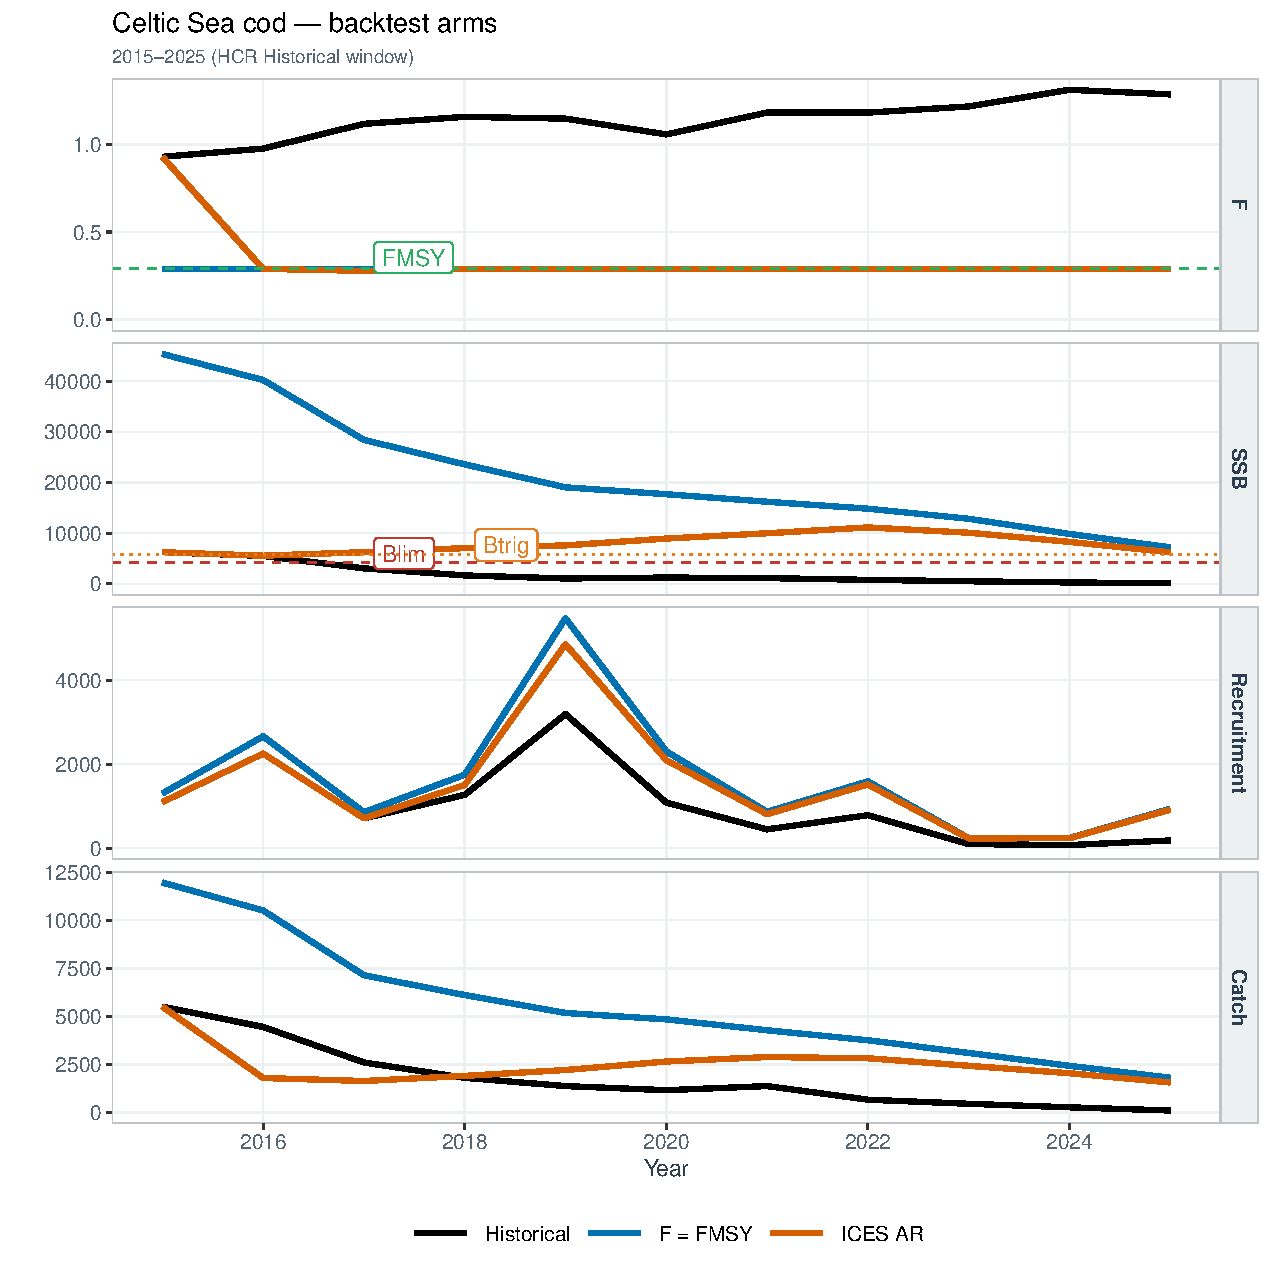
\includegraphics[width=0.49\textwidth]{figs/si/si_backtest_cod.27.7e-k.pdf}%
\hfill
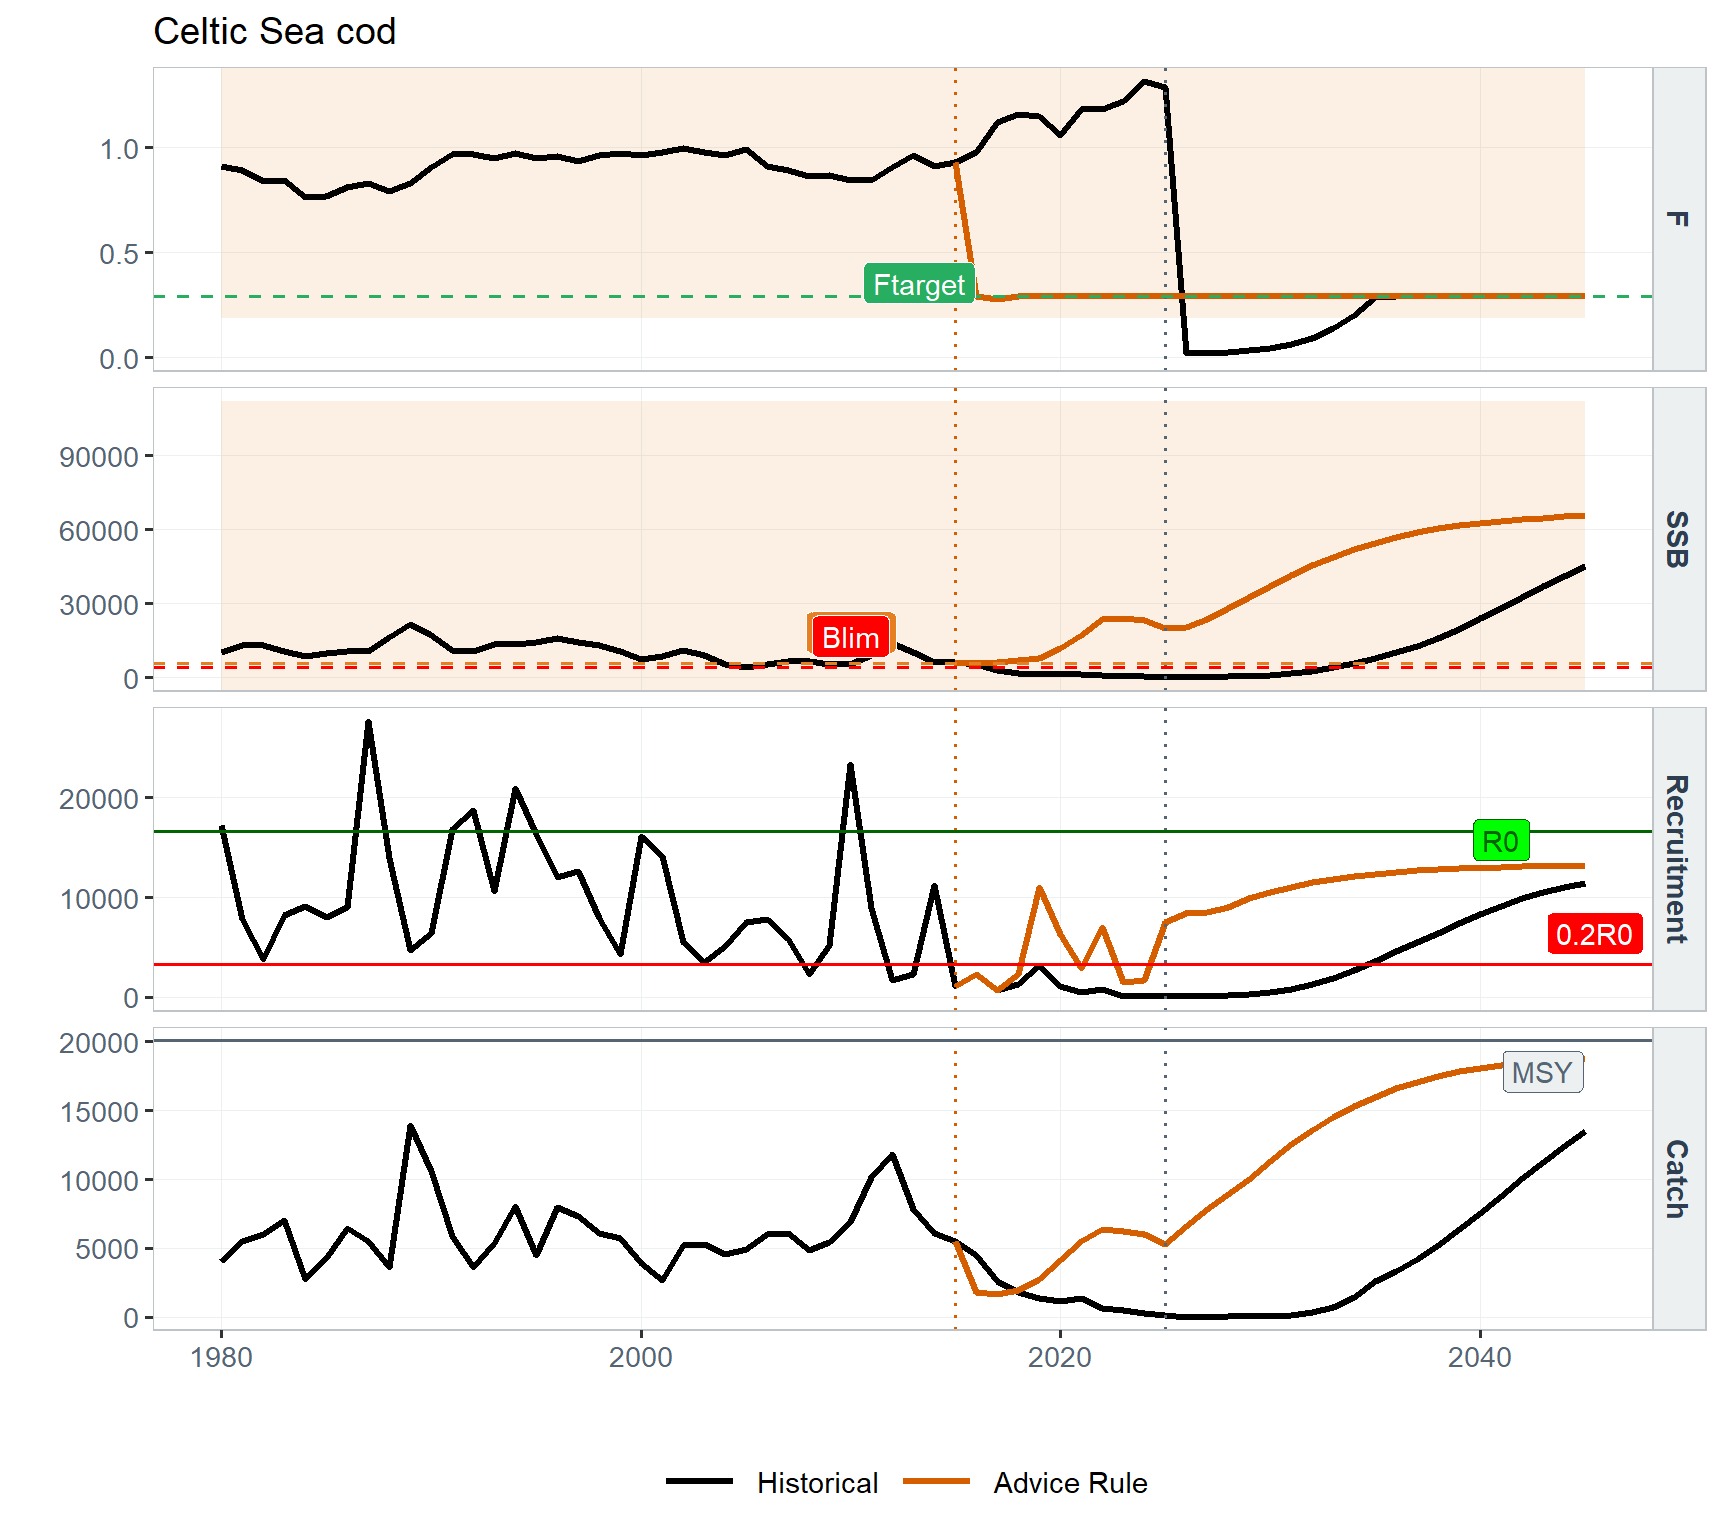
\includegraphics[width=0.49\textwidth]{figs/06.0_report-traj-3.png}
\caption{Outcome pattern~1: Celtic Sea cod. Left: backtest window
(Historical, open-loop $\Fmsy$ benchmark, Advice rule). ICES $\Blim$
(dashed) and $\Btrig$ (dotted) on SSB; $\Ftar$ (dashed) on $\bar F$.
Right: Future rebuild from the Historical and Advice-rule terminal
states; $\Btrig$ met from the Advice-rule start, OM $\Bmsy$ not met in
20 years. Reference OM; mean recruitment.}
\label{fig:hero}
\end{figure}

\begin{figure}[htbp]
\centering
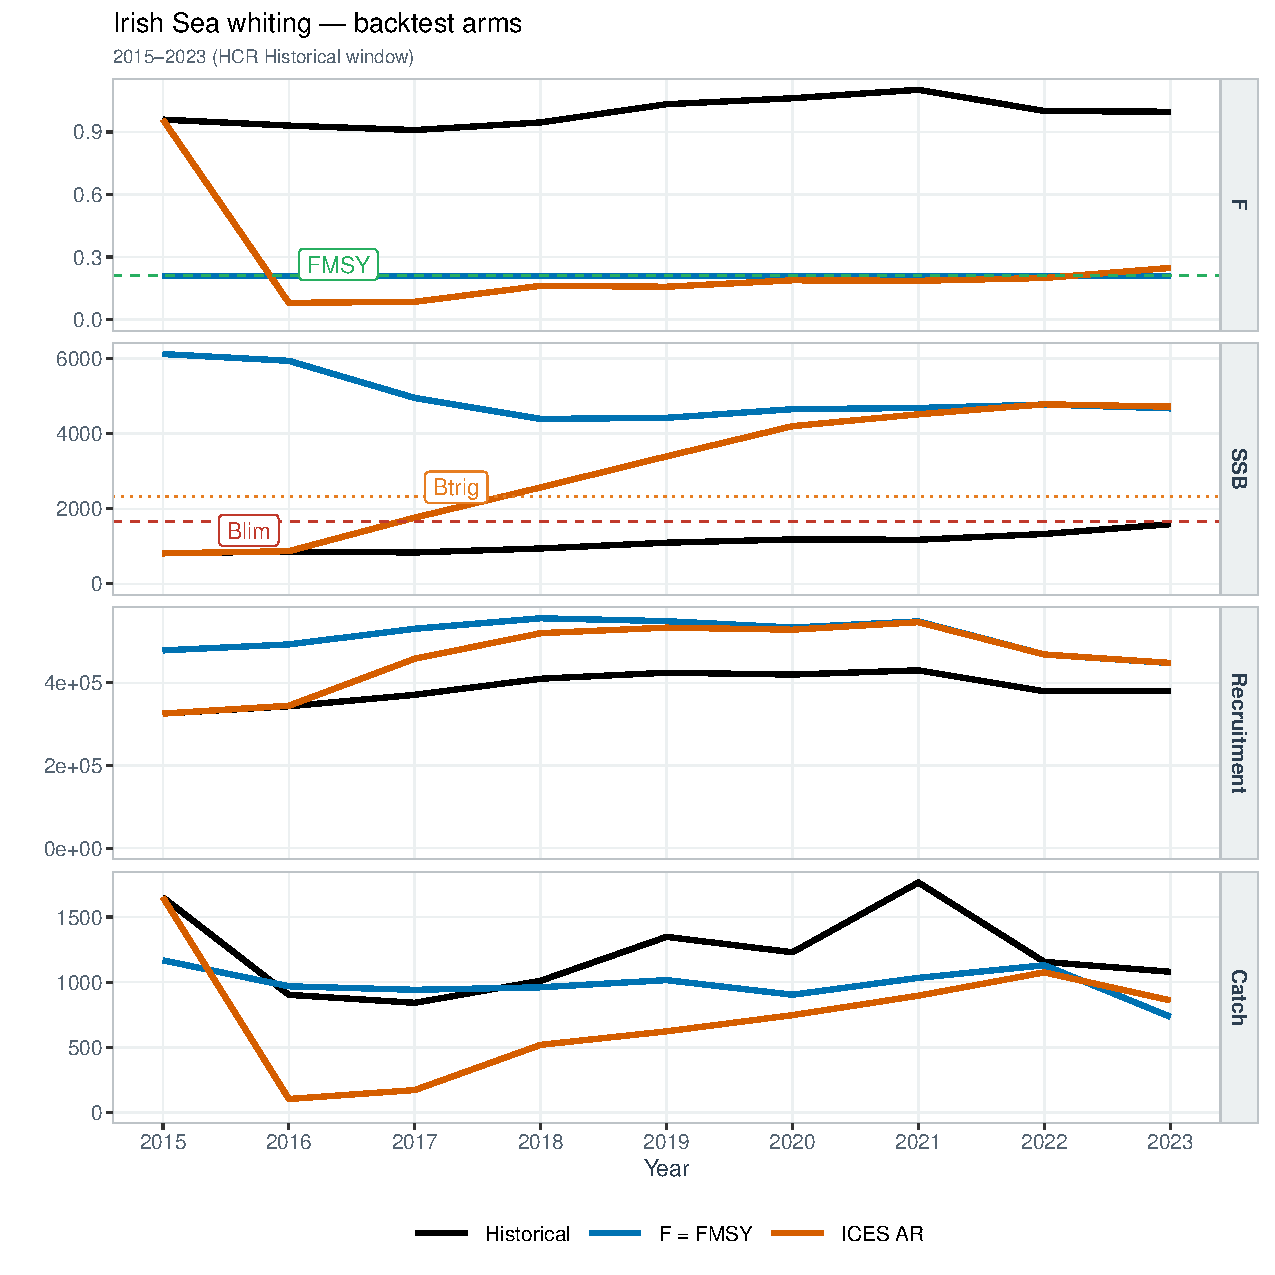
\includegraphics[width=0.49\textwidth]{figs/si/si_backtest_whg.27.7a.pdf}%
\hfill
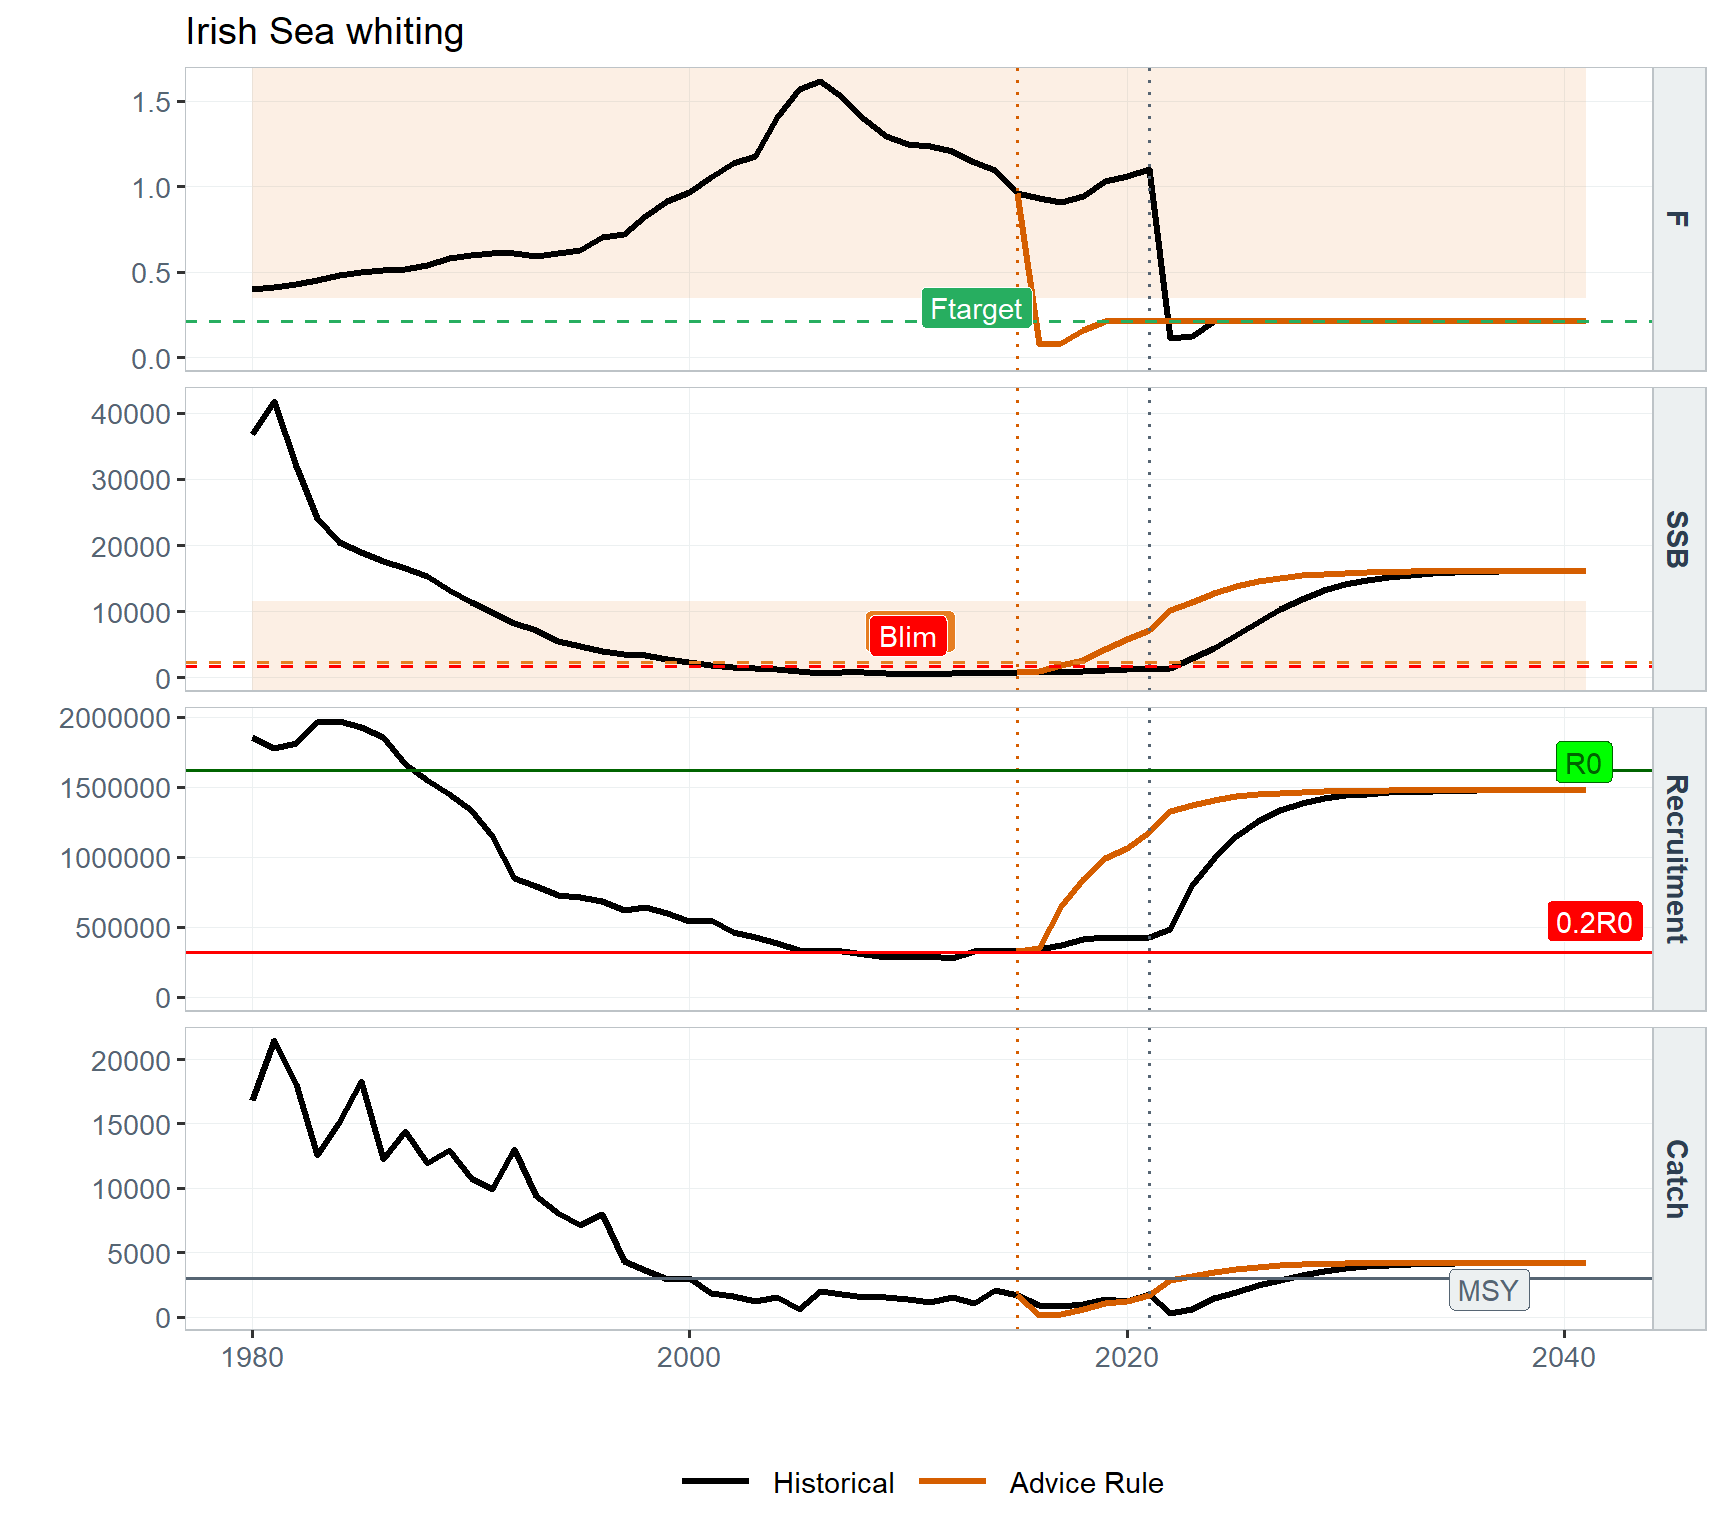
\includegraphics[width=0.49\textwidth]{figs/06.0_report-traj-2.png}
\caption{Outcome pattern~1: Irish Sea whiting. Left: backtest window
(Historical, open-loop $\Fmsy$ benchmark, Advice rule; conventions as in
Figure~\ref{fig:hero}). Right: Future rebuild; already above $\Btrig$
and OM $\Bmsy$ at the Advice-rule start. Reference OM; mean
recruitment.}
\label{fig:hero-whg}
\end{figure}

\begin{figure}[htbp]
\centering
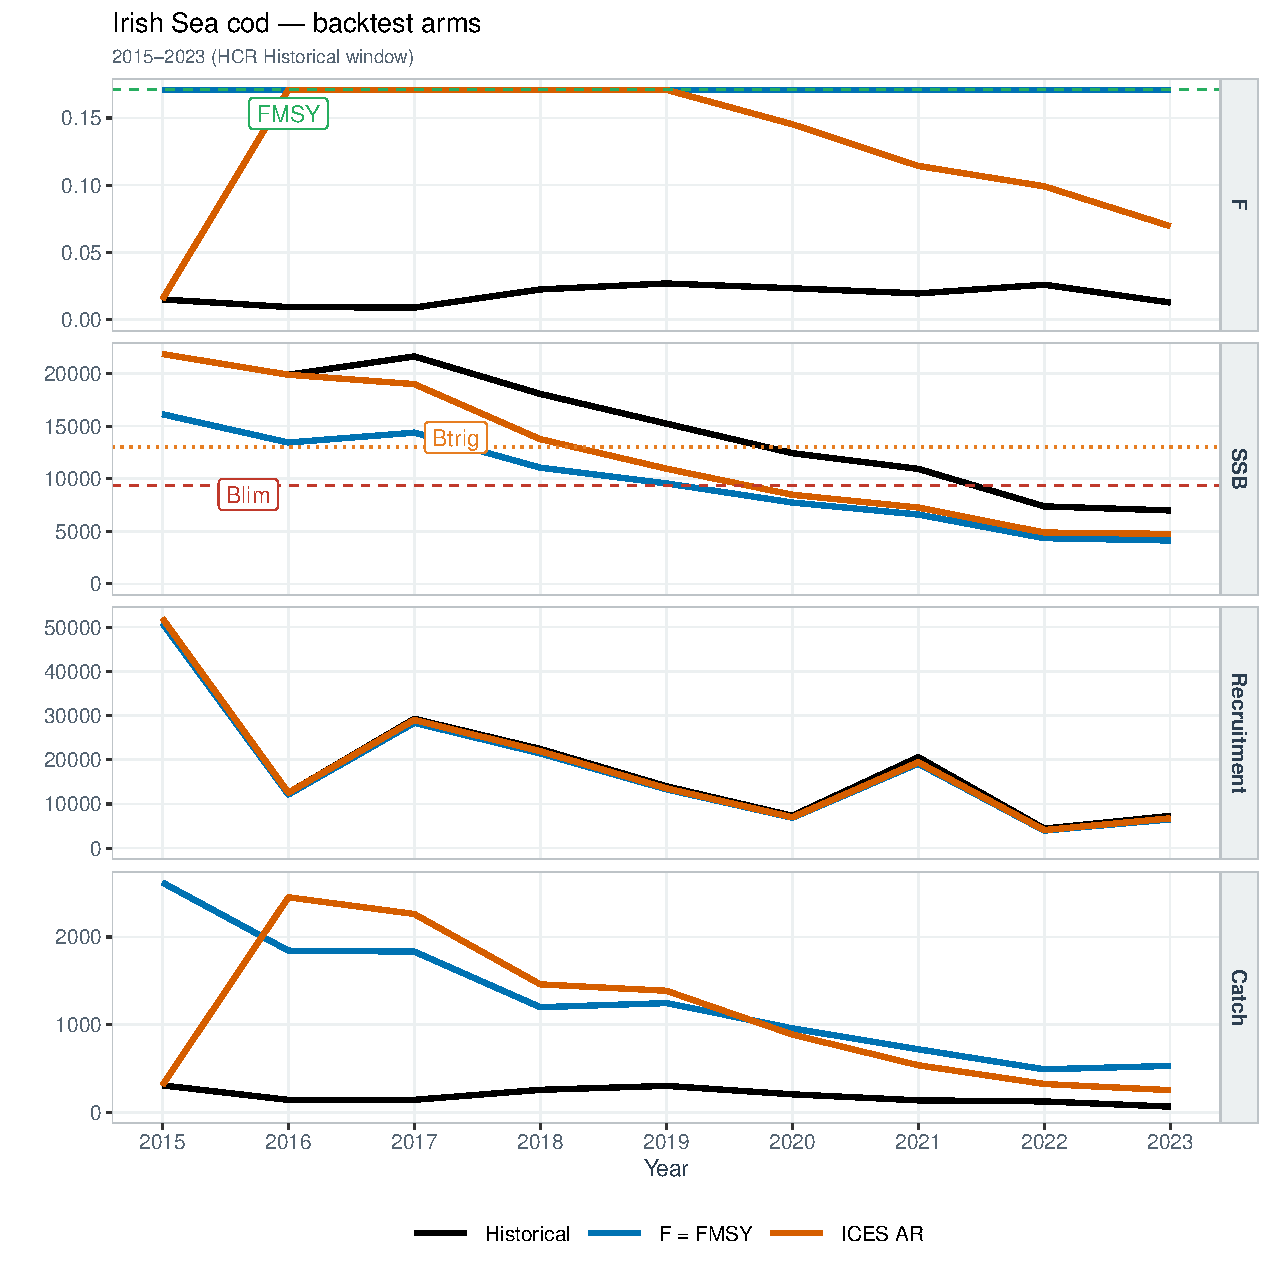
\includegraphics[width=0.49\textwidth]{figs/si/si_backtest_cod.27.7a.pdf}%
\hfill
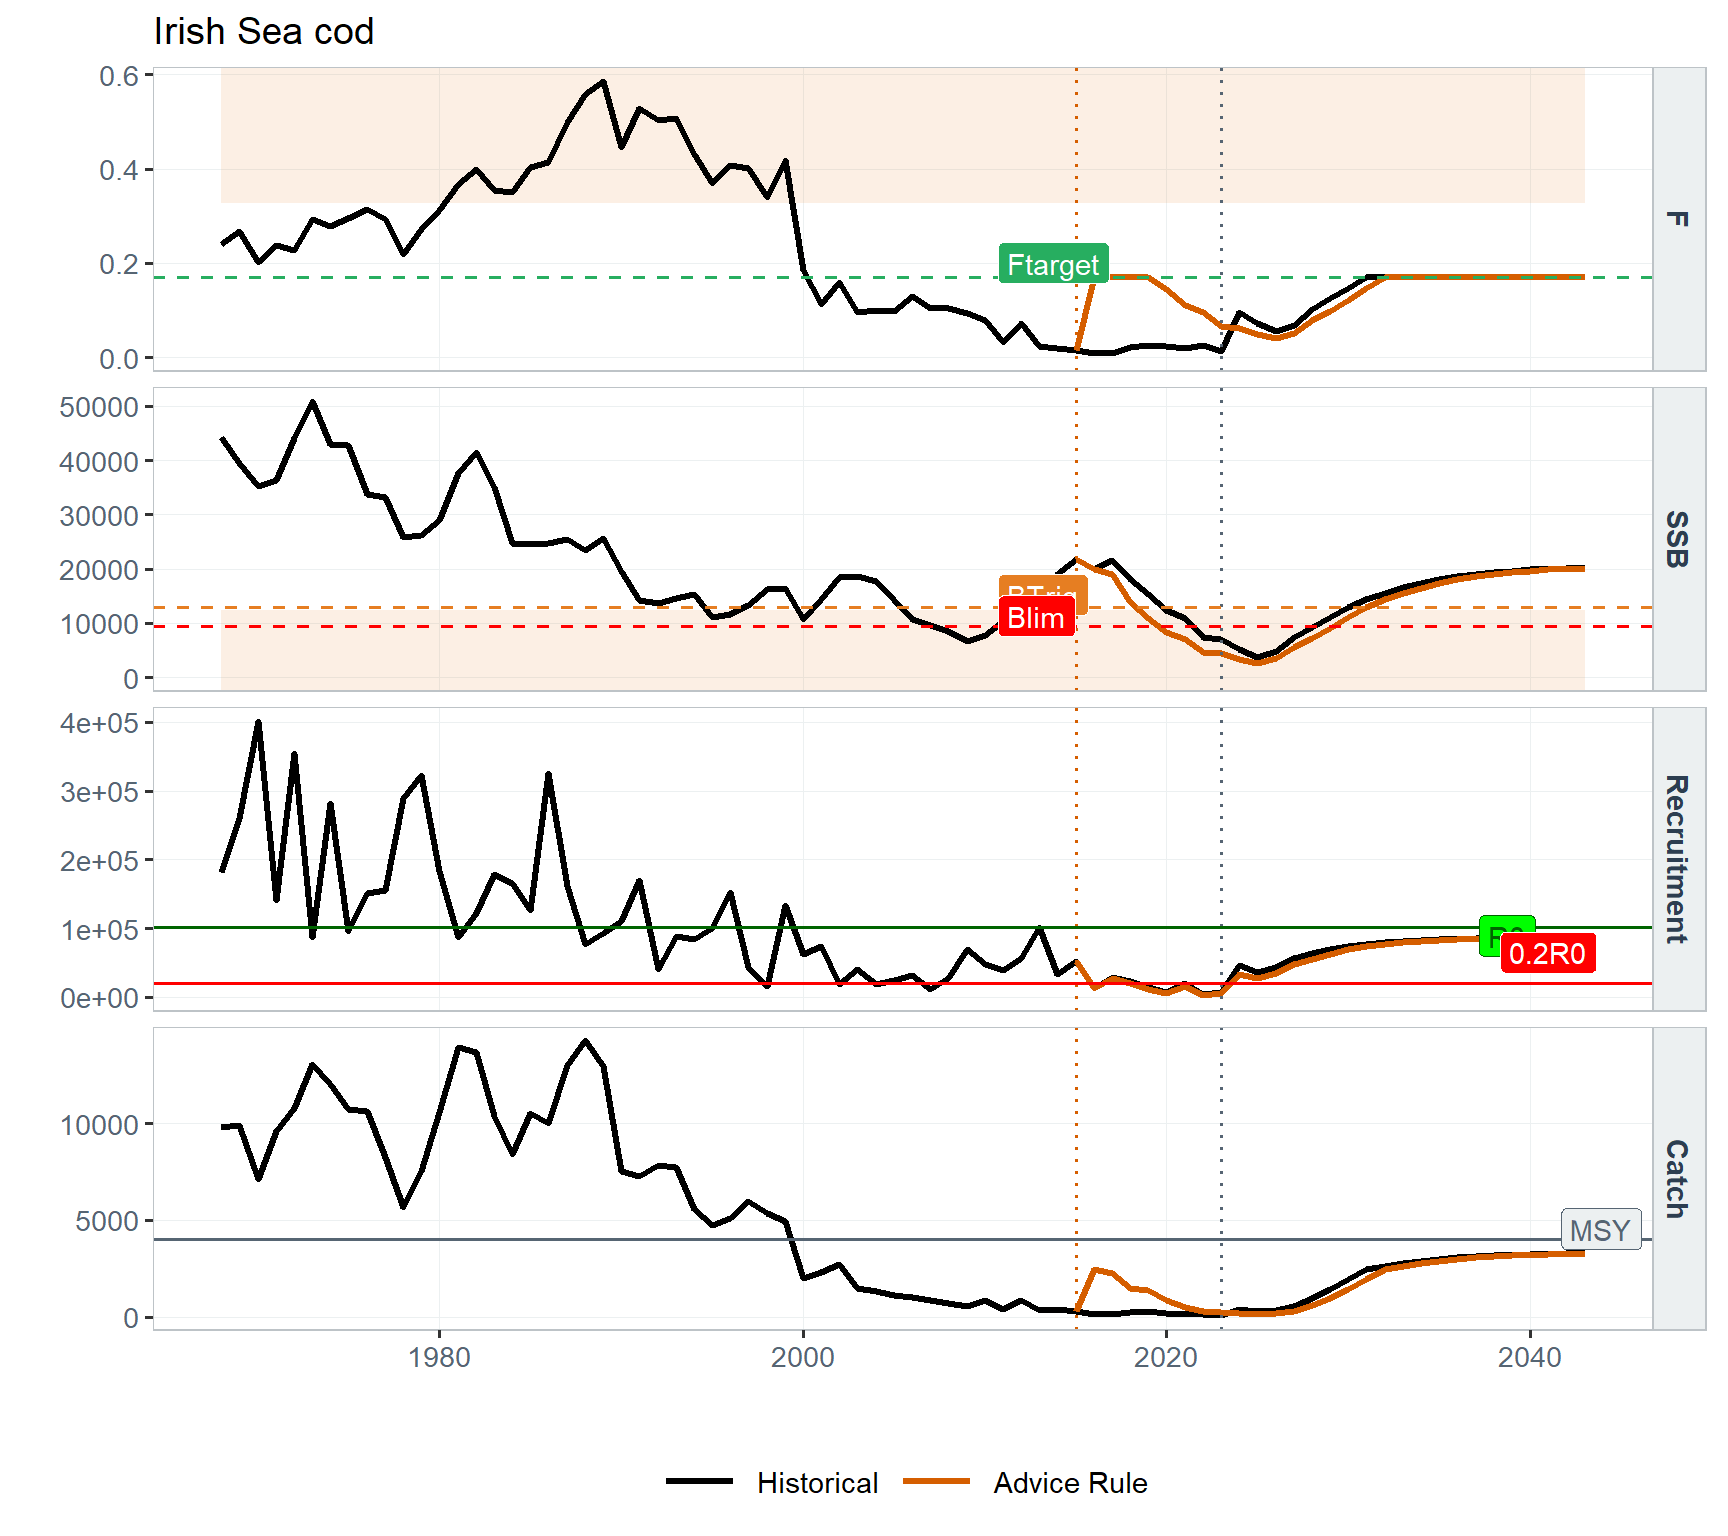
\includegraphics[width=0.49\textwidth]{figs/06.0_report-traj-1.png}
\caption{Outcome pattern~2: Irish Sea cod. Left: backtest window
(Historical, open-loop $\Fmsy$ benchmark, Advice rule; conventions as in
Figure~\ref{fig:hero}). Right: Future rebuild; OM $\Bmsy$ reached before
$\Btrig$. Reference OM; mean recruitment.}
\label{fig:pattern2}
\end{figure}

\begin{figure}[htbp]
\centering
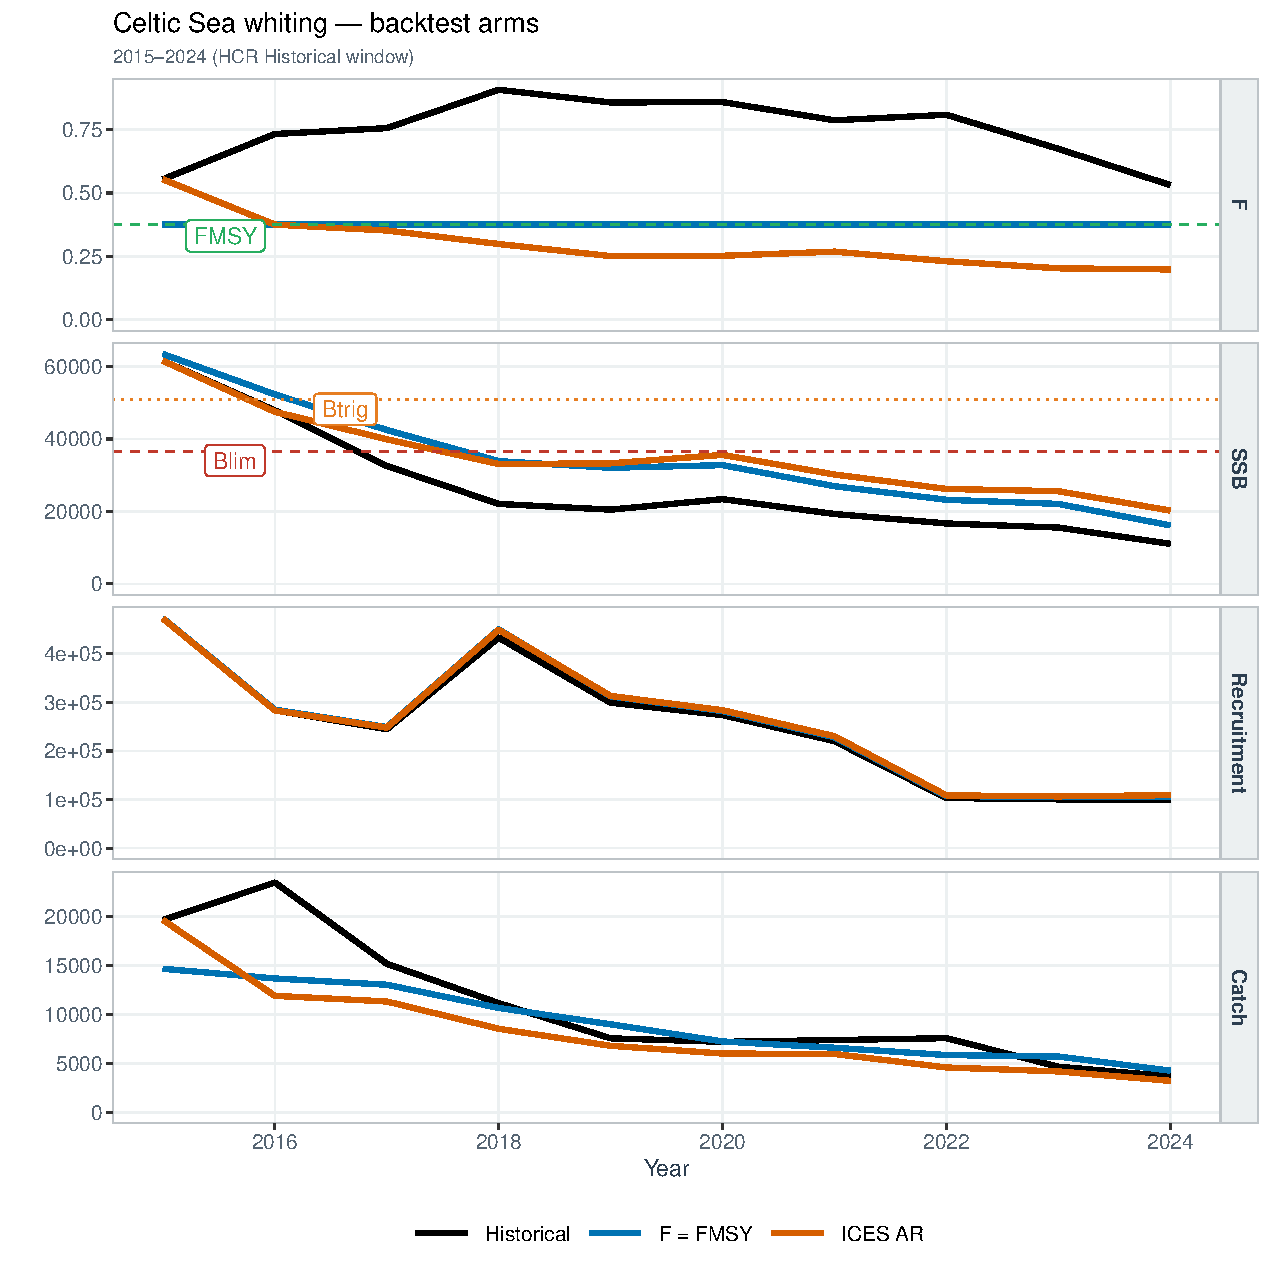
\includegraphics[width=0.49\textwidth]{figs/si/si_backtest_whg.27.7b-ce-k.pdf}%
\hfill
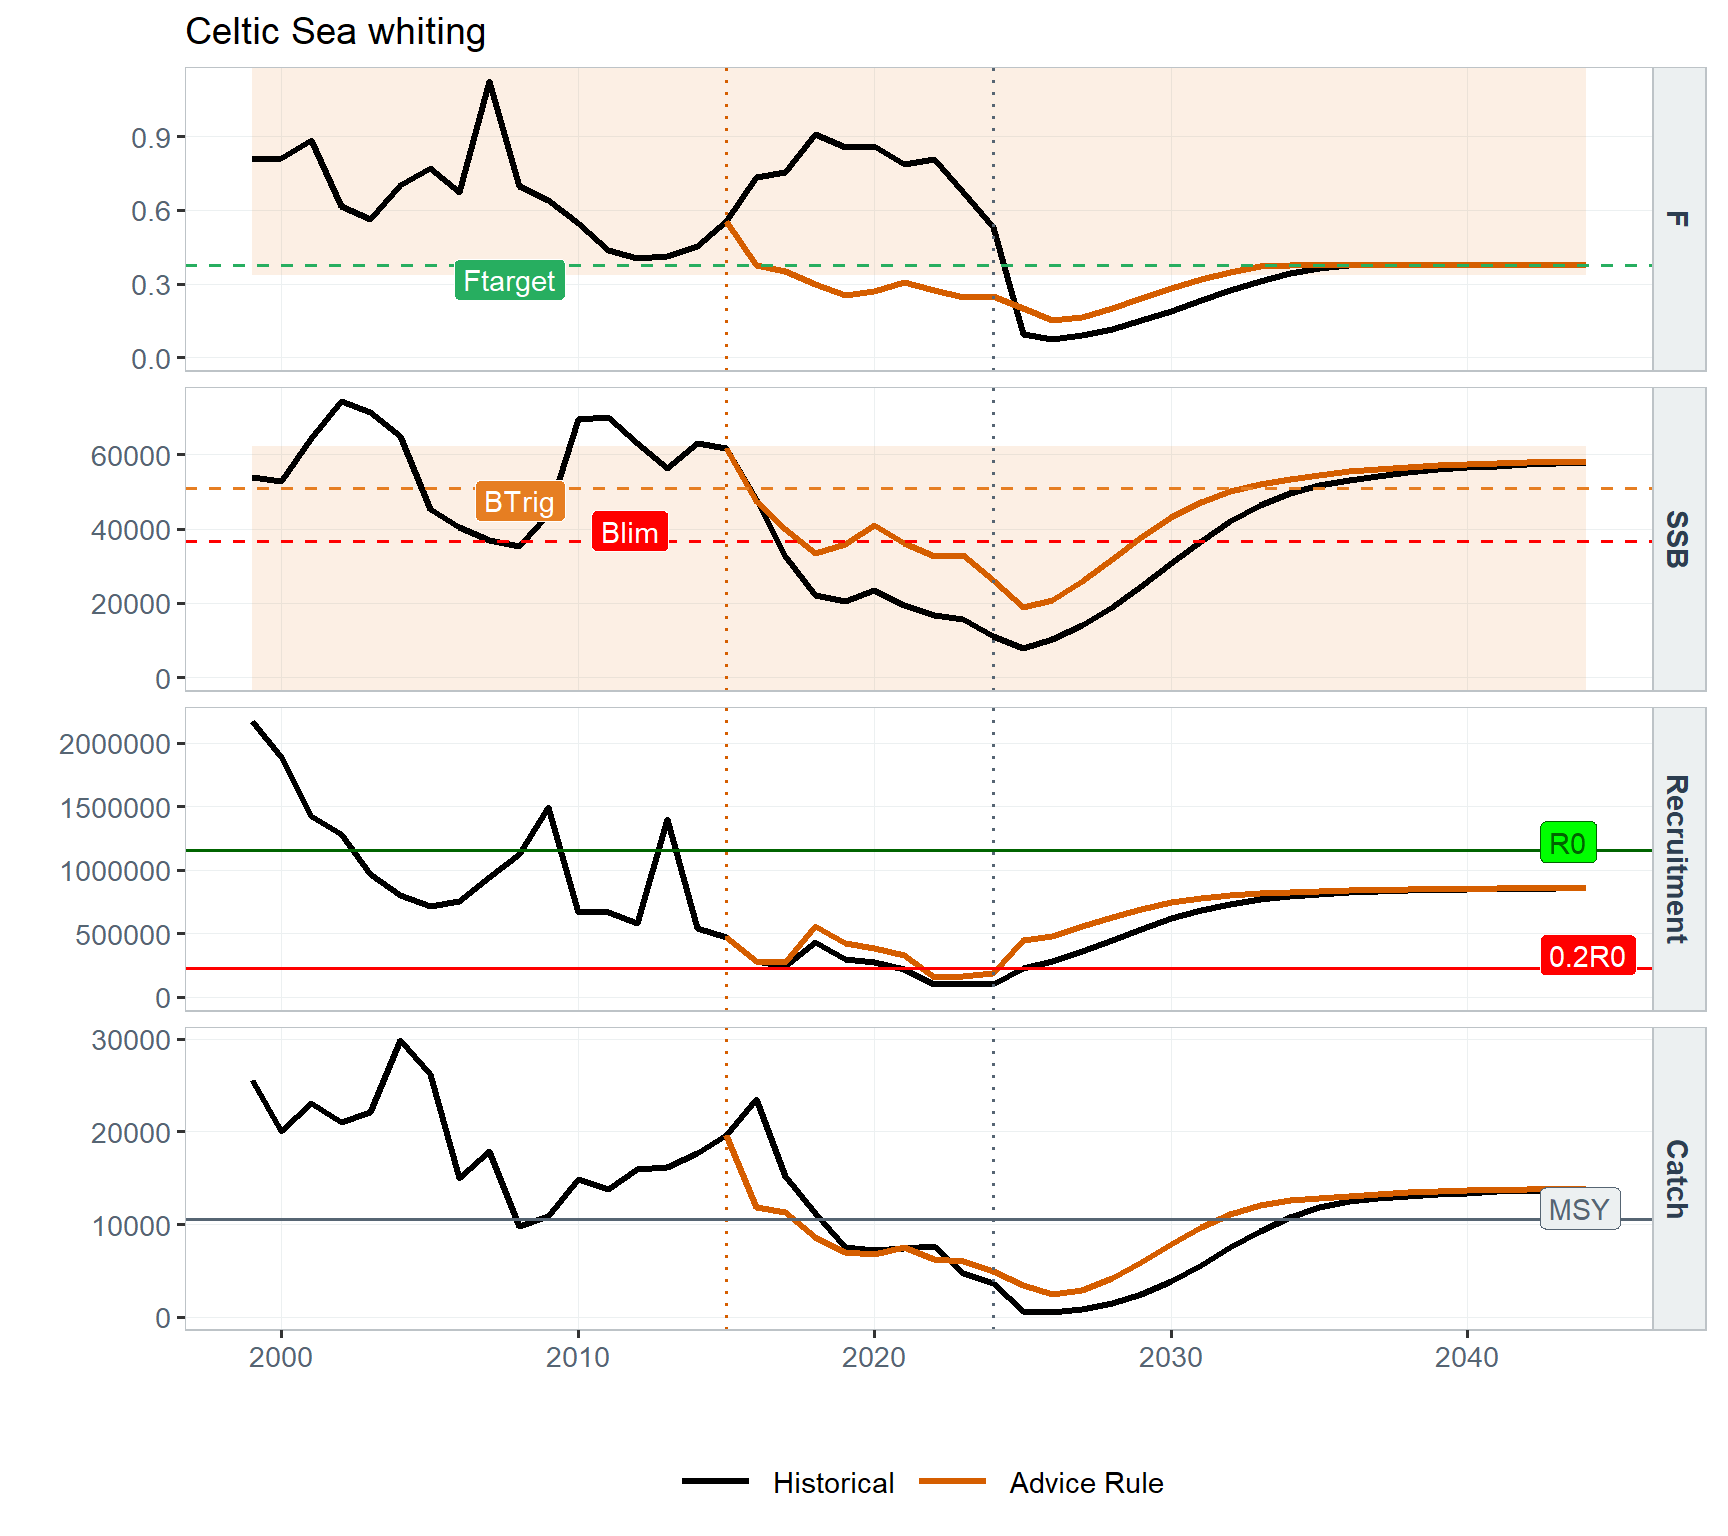
\includegraphics[width=0.49\textwidth]{figs/06.0_report-traj-4.png}
\caption{Outcome pattern~3: Celtic Sea whiting. Left: backtest window
(Historical, open-loop $\Fmsy$ benchmark, Advice rule; conventions as in
Figure~\ref{fig:hero}). Right: Future rebuild; $\Btrig$ not reached in
20 years, OM $\Bmsy$ reached in 16--18 years. Reference OM; mean
recruitment.}
\label{fig:pattern3}
\end{figure}

%==============================================================================
\section{Discussion}
\label{sec:discussion}
%==============================================================================

\subsection{Implementation, rule, and scoring}
\begin{itemize}
  \item The claim is about following the ICES Category~1 \emph{rule} as
        coded (Advice rule vs Historical). Open-loop $\Fmsy$ is a
        no-feedback reference used to interpret that rule; because it
        starts earlier, it does not cleanly isolate hockey-stick shape,
        and it is not a second management option under test. Advice
        rule vs Historical still mixes the HCR with whatever drove
        realised $F$ away from $\Ftar$.
  \item Outcome pattern~1 (overfishing): implementation of a higher $F$
        than the rule prescribed is sufficient to explain remaining below
        trigger. The benchmark moving in the same direction as the HCR
        suggests that $F$ level, rather than the trigger slope, is the
        missing piece. Celtic Sea cod and Irish Sea whiting.
  \item Outcome pattern~2 (opposite sign): Irish Sea cod. Part of the
        shortfall of realised $F$ relative to the coded rule may reflect
        advice as issued; mixed-fishery choke is a plausible mechanism,
        not a result of this backtest.
  \item Outcome pattern~3 (the two yardsticks disagree, in either
        direction). Where OM $\Bmsy$ exceeds $\Btrig$, clearing the
        trigger does not imply MSY biomass: Celtic Sea cod clears
        $\Btrig$ but does not reach OM $\Bmsy$ within 20 years.
        Regionally, median $\Btrig\approx 0.6\,\Bmsy$
        \citep{winker2026rebuilding}, so clearing the trigger need not
        imply that OM $\Bmsy$ is met. Where OM $\Bmsy$ lies below
        $\Btrig$, the reverse holds: Celtic Sea whiting reaches OM
        $\Bmsy$ while remaining below trigger, and following the rule is
        not sufficient, under this stock--recruitment relationship and
        these residuals, to satisfy $\Btrig$. The open-loop check shows
        the same shortfall, so for whiting this is a scoring result under
        the realised productivity (a single fixed replay), not an
        argument that a different ICES $F$ process would have cleared the
        trigger.
  \item Evidence: Tables~\ref{tab:results-current}
        and~\ref{tab:results-future}; Figures~\ref{fig:hero},
        \ref{fig:hero-whg}, \ref{fig:pattern2}, and~\ref{fig:pattern3}.
\end{itemize}

\subsection{Mixed fisheries and choke species}
Irish Sea cod has been managed as a recovery/choke stock, and Celtic Sea
mixed gadoid TACs can bind the most depleted species. This paper does
not model fleet technical interactions, which is a limitation of scope
rather than an unfinished analysis for the present deliverable.

\subsection{What this backtest is not}
This deliverable is a perfect-information backtest (true OM SSB;
residual replay; zero implementation error). Historical, Advice rule, and
open-loop $\Fmsy$ are not three management procedures in an MSE: the
Advice-rule arm is a closed-loop HCR on true SSB, and the open-loop arm
is a no-feedback constant-$F$ reference. The analysis is a historical
backtest of this HCR: not tuning of a management procedure, not a search
over control points, and not an MSE of climates that have not been
observed. It is not climate attribution: residuals are the productivity
history replayed, not a response to temperature. It is not a
contemporaneous reconstruction of advised catch or TACs: advised versus
reported catch is used only for screening. The demonstration excludes
stocks whose benchmark or reference-point basis is not comparable with
the gadoid SAG $\Btrig$. Finally, it does not use short-cut assessment
error or MASE hindcasts of indices.

\subsection{When the backtest transfers}
The design transfers wherever an advice rule can be stated as an HCR,
an OM can be conditioned on an assessment, and observed productivity can
be held fixed while $F$ processes are contrasted. The transferable
products are the closed-loop versus Historical contrast, the subordinate
open-loop $\Fmsy$ benchmark as a no-feedback reference, and dual scoring
against operational control points and OM reference points. What does
not transfer automatically is the mix of outcome patterns: other
ecoregions, other HCRs, or other stock--recruitment and residual
histories may yield only one of the three patterns, or none.
Mixed-fishery constraints and structural uncertainty in the OM remain
stock- or system-specific limits on interpretation (see
Section~\ref{sec:next}). The Celtic and Irish Sea gadoids are a
demonstration that those outcome patterns can co-occur under one advice
framework; they are not the product the methods are built to serve.

%==============================================================================
\section{Conclusions}
\label{sec:conclusions}
%==============================================================================

\begin{itemize}
  \item The backtest separates implementation, rule, and scoring under
        fixed productivity---a contrast transferable to other
        Category~1 (and analogous) advice rules.
  \item Outcome pattern~1: for Celtic Sea cod and Irish Sea whiting,
        which were subject to overfishing, perfect implementation of the
        ICES Category~1 rule as coded would have rebuilt SSB above
        $\Btrig$ by the terminal year.
  \item Outcome pattern~2: for Irish Sea cod the opposite is true:
        following the single-stock rule as coded would have reduced
        terminal SSB relative to history.
  \item Outcome pattern~3: ICES control points and OM MSY reference
        points are different yardsticks that can disagree in either
        direction. Celtic Sea cod clears $\Btrig$ without reaching OM
        $\Bmsy$ within 20 years; Celtic Sea whiting reaches OM $\Bmsy$
        within 16--18 years without clearing $\Btrig$.
  \item Corrective effort therefore may not be aimed only at
        ``implementation''. We hypothesise that scoring conventions and
        mixed-fishery constraints matter as much; the latter are not
        modelled here.
  \item The open-loop $\Fmsy$ trajectory is a no-feedback reference, not
        a recommended alternative harvest policy.
\end{itemize}

%==============================================================================
\section{Next steps}
\label{sec:next}
%==============================================================================

The analyses above complete the contracted historical closed-loop
backtest under perfect information. The items below are optional
enhancements for peer-review readiness and possible further funding.
They are not unfinished promises of the present deliverable, and they are
not required to interpret the Current and Future results reported here.

\begin{enumerate}
  \item \textbf{Multiple operating models for stock--recruit /
        structural uncertainty.}
        This draft reports a single reference OM (Beverton--Holt with the
        coded $R_0$ prior). A journal version would report a small set of
        alternative stock--recruit formulations on the same biology,
        holding ICES HCR inputs fixed, to show whether the three outcome
        patterns are robust to structural uncertainty or are
        hypothesis-specific. That would change interpretation from ``under
        this OM'' to ``across a stated OM set'', without changing the
        Historical versus Advice-rule design.

  \item \textbf{Observation-error model generating CPUE and related
        indices.}
        The perfect-information short-cut feeds true OM SSB to the HCR.
        An observation-error model (OEM) that generates survey or CPUE
        indices---and related assessment inputs---from OM numbers-at-age
        would supply the data stream an assessment needs. That step is
        what makes a full management procedure possible; it does not by
        itself change the residual-replay productivity, but it replaces
        perfect information with observation noise.

  \item \textbf{Full management procedure with SAM as the assessment
        OEM.}
        With an OEM in place, the same ICES hockey-stick can be run as a
        closed-loop management procedure in which a state-space assessment
        model (SAM) is fitted each advice year and the HCR sees estimated
        rather than true SSB. Reference OM, ICES control points, residual
        replay, open-loop benchmark, and stock set would stay as here;
        what changes is assessment error inside the loop. Probabilistic
        summaries (e.g.\ $P(\mathrm{SSB}<\Blim)$) become natural once
        multiple iterations are available.
\end{enumerate}

Closely related items already flagged in the manuscript that would travel
with that upgrade path include mixed-fishery / choke constraints (not
modelled here) and an advised-catch trajectory to separate choke or
recovery TACs from an $\Ftar$--OM~$\Fmsy$ mismatch. Those remain outside
the contracted perfect-information scope.

\bibliographystyle{apalike}
\bibliography{refs}

%==============================================================================
% AUTHOR NOTES (not printed)
%==============================================================================
%
% --- Funder-draft status ---
% This PDF is the contracted deliverable: perfect-information residual-
% replay Historical vs Advice rule, open-loop FMSY=Ftar benchmark, dual
% scoring, four stocks, reference OM (bh3). Peer-review upgrades (multiple
% OMs / SRR; OEM for CPUE; SAM inside MP) live only in sec:next.
%
% --- Suggested figures and tables (max 5 figures, 2 tables) ---
% fig:design --- TikZ schematic in figs/design_schematic.tex.
% fig:hero --- Celtic Sea cod: SI backtest + 06.0 traj-3.
% fig:hero-whg --- Irish Sea whiting: SI backtest + 06.0 traj-2.
% fig:pattern2 --- Irish Sea cod: SI backtest + 06.0 traj-1.
% fig:pattern3 --- Celtic Sea whiting: SI backtest + 06.0 traj-4.
% tab:results-current / tab:results-future --- provisional numbers from
%   the deterministic bh3 run (paper.tex / 06.0); four stocks only.
%
% --- Review checklist (funder draft) ---
% [x] Methods/Intro/Abstract/Discussion/Conclusions describe only what
%     was done (perfect-info short-cut).
% [x] Next steps lists (i)--(iii) as optional peer-review upgrades.
% [x] No "planned SAM", "when OEM is ready", or multiple-SRR roadmap in
%     main sections.
% [x] Notation: Ftar = HCR; Fmsy/Bmsy = OM; Btrig upright MSY Btrigger;
%     open-loop uses published ICES FMSY = Ftar.
% [ ] Freeze figures from a clean re-knit before journal submission.
% [ ] Author list / funding acknowledgement when required.
%
% --- Code to run, skip list, and gaps ---
% See tex/code-to-run.md.

\end{document}
